\section{Spracovávané Dáta}

Budeme spracovávať dáta pacientov, ktorý užívali dva rôzne lieky (nikdy nie naraz) proti primárnej chorobe. Máme k dispozícii dáta o vzorke 10 000 pacietov.


K dispozícii máme, aký liek bol podávaný pacientovi a aký účinok to malo na jeho primárne ochorenie. Ďalej máme k dispozícii základné fyzické proporcie pacienta ako: vek, index telesnej hmotnosti a priemerný krvný tlak. Je nám známa taktiež anamnéza pacienta (výskyt sekundárnych chorôb pred a po liečbe a iná nešpecifikovaná medikácia).

ROZDELENIE VEK BMI TLAK GRAFY A TABUĽKY (štatistická významnosť 0.05) ???


\begin{figure}[h!]
	\centering
  		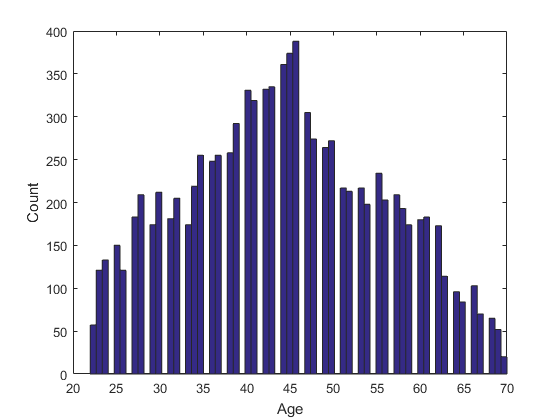
\includegraphics[width=1.0\textwidth]{ages.png}
  	\caption{Histogram Vekov}
\end{figure}




\begin{table}[h!]
\centering
\label{vek}
\begin{tabular}{c|cccccc}
\hline
\textbf{Vek}             & 24- & 25-34 & 35-44 & 45-54 & 55-64 & 65+ \\ \hline
\textbf{Počet Pacientov} & 311 & 1828  & 2986  & 2722  & 1759  & 394 \\ \hline
\end{tabular}
\caption{Vek pacientov}
\end{table}